% =====================================================================
%  Passaggio al limite sotto il segno di derivata -- lezione 2
% =====================================================================

% [1:12:12]
\section{Passaggio al limite sotto il segno di derivata}

\subsection{Perché il problema è più delicato}

La domanda analoga per le derivate è: vale
\[
\frac{d}{dx}\Big(\lim_{n\to\infty} f_n(x)\Big)
=\lim_{n\to\infty}\frac{d}{dx}f_n(x)\,?
\]

\paragraph{In aula.} Qui la situazione è molto più complessa che per l'integrale. Nel
caso dell'integrale gli oggetti $I_n$ erano \emph{numeri}: la convergenza era quella
di una successione numerica e non c'era ambiguità. Le derivate $f_n'$ sono invece
\emph{funzioni}, e una successione di funzioni può convergere in modi diversi, o non
convergere affatto. Può succedere che la funzione limite non sia derivabile anche se
tutte le $f_n$ lo sono; che le derivate non ammettano limite; che i due membri
esistano ma siano diversi. Servono quindi più ipotesi. I tre esempi che seguono
servono a capire quali.

% [1:16:37]
\subsection{Esempio 1: il limite può non essere derivabile}

\[
f_n(x)=\sqrt{x^2+\frac{1}{n}},\qquad x\in\mathbb{R}.
\]
Ogni $f_n$ è derivabile infinite volte su $\mathbb{R}$: il radicando è strettamente
positivo grazie al termine $1/n$, quindi il problema della radice in zero non si
presenta. Il limite puntuale è
\[
\lim_{n\to\infty} f_n(x)=|x|=f(x),
\]
che non è derivabile in $x=0$ (figura~\ref{fig:05}).

La convergenza è addirittura uniforme. Infatti, razionalizzando,
\[
\big|f_n(x)-|x|\big|
=\sqrt{x^2+\tfrac1n}-|x|
=\frac{1/n}{\sqrt{x^2+\tfrac1n}+|x|},
\]
quantità decrescente in $|x|$: il $\sup$ si ottiene in $x=0$ e vale
$\dfrac{1/n}{\sqrt{1/n}}=\dfrac{1}{\sqrt n}\to 0$.

\BoxBlue{Osservazione}{}{%
Dunque la sola convergenza uniforme delle $f_n$ non basta:
occorre chiedere qualcosa sulle \emph{derivate}.
}

\begin{figure}[htbp]\centering
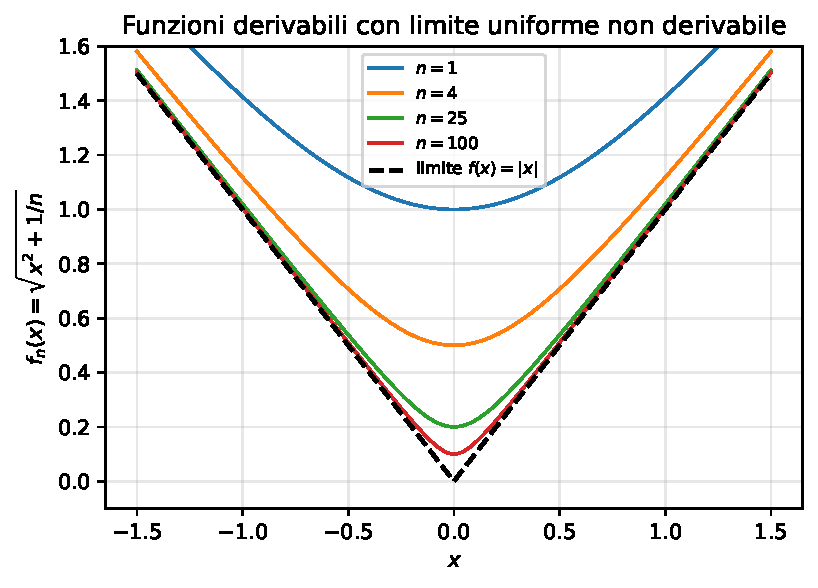
\includegraphics[width=0.6\linewidth]{figure/fig_05}
\caption{Andamento qualitativo di $f_n(x)=\sqrt{x^2+1/n}$: funzioni regolari che
convergono uniformemente a $|x|$, non derivabile in $x=0$.}
\label{fig:05}
\end{figure}

% [1:21:51]
\subsection{Esempio 2: le derivate possono non convergere}

\[
f_n(x)=\frac{\sin(nx)}{n},\qquad x\in\mathbb{R}.
\]
Si ha $f_n\rightrightarrows f\equiv 0$, e la verifica è immediata: $|\sin(nx)|\le 1$,
quindi $|f_n(x)|\le 1/n\to 0$ indipendentemente da $x$. Le $f_n$ sono derivabili
quante volte si vuole, quindi stavolta tutti i presupposti ci sono. Però
\[
f_n'(x)=\cos(nx),
\]
che per $x$ generico è oscillante e non ammette limite. Nei punti in cui il limite
esiste, per esempio $x=0$, si ha $f_n'(0)=1$ per ogni $n$, mentre $f'(0)=0$: i due
membri esistono ma sono diversi (figura~\ref{fig:06}).

\begin{figure}[htbp]\centering
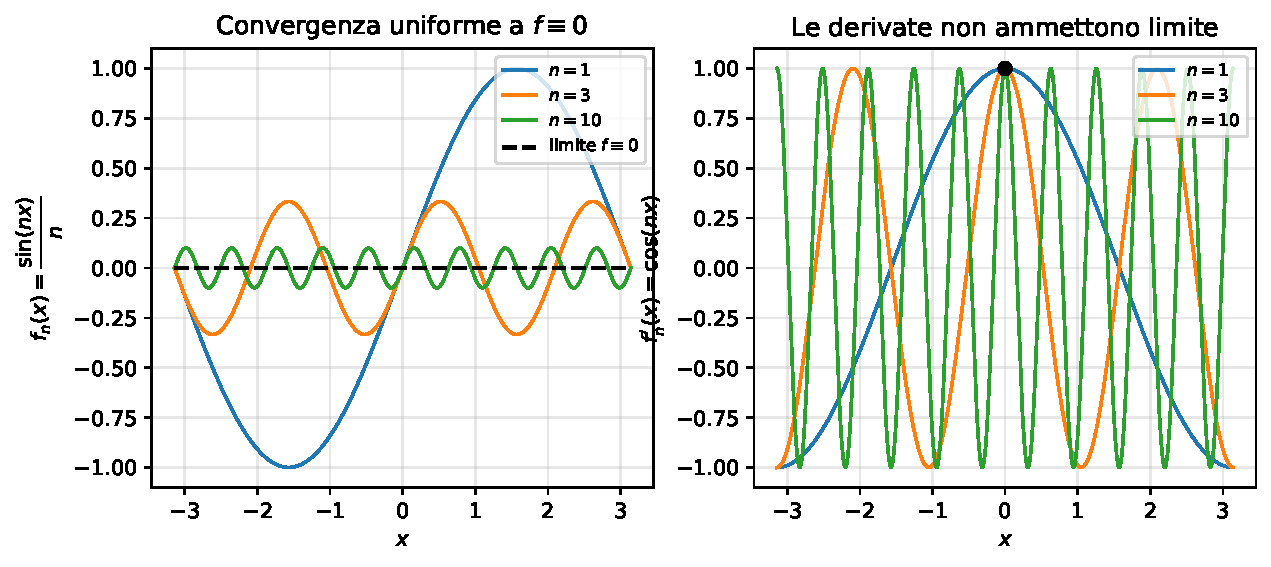
\includegraphics[width=0.85\linewidth]{figure/fig_06}
\caption{Andamento qualitativo di $f_n(x)=\sin(nx)/n$ (a sinistra) e della successione
delle derivate $f_n'(x)=\cos(nx)$ (a destra): convergenza uniforme delle $f_n$, nessun
limite per le derivate.}
\label{fig:06}
\end{figure}

% [1:25:48]
\subsection{Esempio 3: le derivate convergono, ma solo puntualmente}

\[
f_n(x)=\frac{x}{1+n^2x^2},\qquad x\in[0,1].
\]
Si ha $f_n\rightrightarrows f\equiv 0$ (per $x=0$ la funzione è nulla; per $x\neq 0$ il
denominatore diverge; la verifica dell'uniformità si fa come negli esempi precedenti),
quindi $f'\equiv 0$. Le derivate esistono per ogni $n$, perché il denominatore non si
annulla mai:
\[
f_n'(x)=\frac{1-n^2x^2}{(1+n^2x^2)^2}.
\]
Stavolta la successione delle derivate \emph{ammette} limite puntuale:
\[
f_n'(x)\longrightarrow
\begin{cases}
0, & x\neq 0,\\
1, & x=0,
\end{cases}
\]
e quindi
\[
\lim_{n\to\infty} f_n'(0)=1\neq 0=f'(0).
\]
Il passaggio al limite non vale. Il limite delle derivate è discontinuo in $0$ mentre
le $f_n'$ sono continue: per il teorema di continuità del limite la convergenza delle
derivate non è uniforme (figura~\ref{fig:07}).

\begin{figure}[htbp]\centering
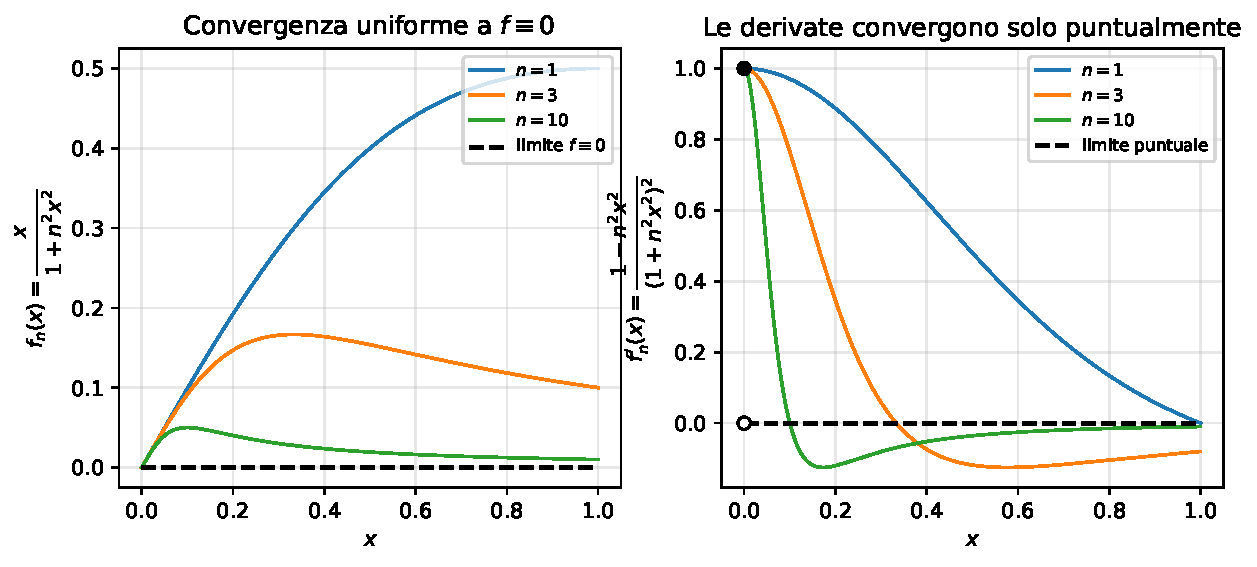
\includegraphics[width=0.85\linewidth]{figure/fig_07}
\caption{Andamento qualitativo di $f_n(x)=x/(1+n^2x^2)$ (a sinistra) e delle derivate
$f_n'(x)=(1-n^2x^2)/(1+n^2x^2)^2$ (a destra) su $[0,1]$: il limite delle derivate è
discontinuo in $x=0$.}
\label{fig:07}
\end{figure}

% [1:31:05]
\paragraph{In aula.} Il filo conduttore dei tre esempi è che in nessuno di essi si è
mai chiesto che la successione delle \emph{derivate} converga uniformemente: è questa
l'informazione che manca. Al contrario, nel terzo esempio si vede che quello che fanno
le $f_n$ è quasi irrilevante: sarà sufficiente saperne il comportamento in un solo
punto.

% [1:32:01]
\subsection{Enunciato}

\Teorema{passaggio al limite sotto il segno di derivata}{%
Siano
\begin{enumerate}
  \item $f_n\colon[a,b]\to\mathbb{R}$ con $f_n\in C^1([a,b])$ per ogni $n$;
  \item esista $x_0\in[a,b]$ tale che $\displaystyle\lim_{n\to\infty}f_n(x_0)=L\in\mathbb{R}$;
  \item esista $g\colon[a,b]\to\mathbb{R}$ tale che $f_n'\rightrightarrows g$ in $[a,b]$.
\end{enumerate}
Allora
\begin{enumerate}
  \item[T1)] $f_n\rightrightarrows f$ in $[a,b]$, per una opportuna $f\colon[a,b]\to\mathbb{R}$;
  \item[T2)] $f\in C^1([a,b])$ e $f'=g$, cioè
\end{enumerate}
\begin{equation}
\frac{d}{dx}\Big(\lim_{n\to\infty} f_n(x)\Big)
=\lim_{n\to\infty}\frac{d}{dx}f_n(x).
\end{equation}
}

\BoxBlue{Osservazione}{}{%
$C^1([a,b])$ significa: derivabile con derivata continua.
L'ipotesi $C^1$ si può indebolire chiedendo solo la derivabilità, ma l'enunciato e
soprattutto la dimostrazione diventano sensibilmente più complicati; nei testi si
trova anche quella versione.
}

\BoxBlue{Osservazione}{}{%
L'ipotesi 2 è sorprendentemente debole: delle $f_n$ non si
chiede nulla, se non che convergano \emph{in un solo punto}. L'ipotesi sostanziale è
la 3, la convergenza uniforme delle derivate. Si noti che la convergenza (anche
uniforme) delle $f_n$, che negli esempi c'era sempre, non è servita a nulla.
}

\subsection{Dimostrazione}
% [0:01:19]
Questo è il più complesso dei tre teoremi di passaggio al limite, perché li \emph{usa}
entrambi: il teorema di continuità del limite serve a dire che $g$ è continua, quello di
passaggio al limite sotto il segno di integrale a costruire $f$. Chi non conosce i primi
due non può dimostrare questo.

\paragraph{Passo 1: costruire $f$.} La funzione $f$ non è data, va costruita: le ipotesi
danno un'informazione sulla successione in un solo punto, $x_0$. Poiché $f_n\in C^1$
— ipotesi che qui viene sfruttata in modo essenziale — la sua derivata $f_n'$ è continua
e quindi integrabile: per il teorema fondamentale del calcolo integrale
\begin{equation}
f_n(x)=f_n(x_0)+\int_{x_0}^{x} f_n'(t)\,dt,\qquad x\in[a,b].
\end{equation}
% [0:02:50]
La riscrittura sembra artificiosa — si parte da una funzione che c'è già e la si riscrive
in una forma più complicata — ma è proprio ciò che conviene, perché fa \emph{comparire una
funzione}: il membro di destra ammette limite.
\begin{itemize}
  \item $f_n(x_0)\to L$ per l'ipotesi 2;
  \item $\displaystyle\int_{x_0}^{x} f_n'(t)\,dt\to\int_{x_0}^{x} g(t)\,dt$ per il
  teorema di passaggio al limite sotto il segno di integrale, applicabile grazie alle
  ipotesi 1 e 3 (le $f_n'$ sono continue e convergono uniformemente a $g$).
\end{itemize}
Dunque $f_n$ converge puntualmente alla funzione
\begin{equation}
f(x)=L+\int_{x_0}^{x} g(t)\,dt .
\end{equation}

% [1:41:50]
\paragraph{Passo 2: la tesi T2.} La $g$ è continua, perché è limite uniforme delle
funzioni continue $f_n'$ (teorema di continuità del limite). Allora
$x\mapsto\int_{x_0}^{x} g(t)\,dt$ è la funzione integrale di una funzione continua,
quindi per il teorema fondamentale del calcolo è derivabile con derivata $g(x)$; il
termine $L$ è una costante e ha derivata nulla. Perciò
\[
f'(x)=g(x)\quad\text{in }[a,b],
\]
e poiché $g$ è continua si ha $f\in C^1([a,b])$. Questa è esattamente la tesi T2.
% [0:09:40]
Conviene fissare la distinzione che si è appena usata: se l'integranda è \emph{solo
integrabile}, della funzione integrale si può concludere soltanto la continuità; se
l'integranda è \emph{continua}, si guadagna di più, cioè la derivabilità con derivata
l'integranda — ed è precisamente ciò che serve qui.

% [1:45:23]
\paragraph{Passo 3: la tesi T1.} Resta da mostrare che la convergenza $f_n\to f$ è
uniforme. L'idea è maggiorare $|f_n(x)-f(x)|$ con una quantità che non dipende da $x$ e
che tende a zero in $n$. Sottraendo le due rappresentazioni integrali e usando la
disuguaglianza triangolare:
\begin{align*}
0\le |f_n(x)-f(x)|
&\le |f_n(x_0)-L|+\left|\int_{x_0}^{x}\big(f_n'(t)-g(t)\big)\,dt\right|\\
&\le |f_n(x_0)-L|+\int_a^b \big|f_n'(t)-g(t)\big|\,dt\\
&\le |f_n(x_0)-L|+\max_{t\in[a,b]}\big|f_n'(t)-g(t)\big|\cdot(b-a).
\end{align*}
% [0:06:54]
Nel passaggio alla seconda riga il punto delicato è il \emph{doppio modulo}: il valore
assoluto si può portare \emph{dentro} l'integrale (maggiorando), ma quello \emph{fuori} va
lasciato. Il motivo è che gli estremi $x_0$ e $x$ sono in ordine ignoto: se fosse $x<x_0$
l'integrale cambierebbe segno e si starebbe maggiorando una quantità positiva con una
negativa, il che non è lecito. Quando gli estremi sono variabili, dunque, si può mettere
il modulo dentro ma non si può togliere quello fuori.
% [0:08:19]
Solo a questo punto, essendo l'integranda positiva, ci si libera della dipendenza da $x$
\emph{allargando} l'intervallo di integrazione a tutto $[a,b]$.

Il membro di destra \emph{non dipende da $x$}: il primo addendo tende a zero per
l'ipotesi 2, il secondo per l'ipotesi 3. Passando al $\sup$ su $x\in[a,b]$ la
maggiorazione si conserva, quindi
\[
0\le\sup_{x\in[a,b]}|f_n(x)-f(x)|\longrightarrow 0,
\]
cioè $f_n\rightrightarrows f$. $\blacksquare$

Il punto cruciale è proprio che la maggiorazione sia \emph{indipendente da $x$}: solo così
sopravvive al passaggio al $\sup$ e permette di concludere con il teorema dei carabinieri,
senza calcolare alcuna derivata. Se la quantità maggiorante dipendesse da $x$, l'argomento
non funzionerebbe.
